%First, make the design space as large as possible
% tradeoffs/considerations/selection
% 1 or 2 solutions

First, let us list the design decisions. We start with the first decision, namely, how to encode explicit datapaths such that the hardware knows about bypasses. Then is the manner of when in the compilation chain does it actually encode these bypasses.
%TODO: extend with other decisions that are added below.

%TODO: add decision of how to encode the bypass registers. Choice to use register index space or add bits to instruction

%TODO: (is explained at class diagram 3.4.3) add decision for predicate flag instructions, we made getStartOperand to skip flagged instructions. Alternatively, it is also possible to ignore any flag operands that are encountered.
\subsubsection{Encoding datapaths}
The first design decision is how to encode that an operand is forwarded. There are two ways to encode that a source operand comes from the bypass network:
\begin{enumerate}[i.]
  \item Add bits to each instruction to specify that a certain operand comes from the bypass network. It requires three bits per source operands because there are five different bypass sources with a five-stage pipeline. Each instruction may have up to two source operands that can be bypassed. Therefore, this approach requires six additional bits to be added to each instruction.
  \item Use register index space to indicate that an operand comes from the bypass network. This requires at most five registers to be reserved because we have at most five bypass sources.
\end{enumerate} 

We have chosen to use the register index space because the hardware description of the architecture corresponds to that, and because of the nice feature that it does not require any modification to the instruction format.

\begin{figure}[b]
\centering
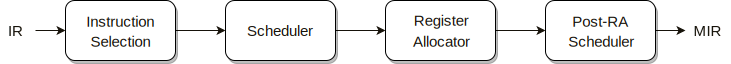
\includegraphics[width=.9\textwidth]{figures/phase_ordering}
\caption{Phase ordering problem.}
\label{fig:phase_ordering}
\end{figure}

\subsubsection{When and how to allocate explicit registers}
Let us start with when to allocate explicit bypass registers. First of all, ideally that would be done before register allocation where we still have virtual registers. The number of virtual registers reduces with each store that is avoided. Thereby, reducing register pressure and relaxing the job for the register allocator.

However, when the register allocator runs out of registers and inserts spill code between two instructions that were already bypassed, this bypass may not be valid anymore and therefore, requiring an additional register to undo that bypass.

Trivially, it is not possible to allocate explicit bypass registers before scheduling, because the order of instructions is not known at that time. So, alternatively it can be done after register allocation. However, the physical registers that are freed by dead result elimination are not exploited when doing this after RA, therefore, not gaining from reduced register pressure. Moreover, if spill code was necessary it has already been inserted when doing this after register allocation. Therefore, it may have redundant spill code.

To summarize, ideally we exploit explicit datapaths before register allocation to gain from reduced register pressure. But alternatively, it can be done after register allocation which may potentially have redundant spill code.\\



How to exploit explicit register allocation is a very broad question, in fact this is the main goal of this assignment. Lets split up in two categories of approaches:
\begin{enumerate}[i.]
  \item One way to exploit explicit datapaths is to group instructions close to their use. Moreover, if an instruction is strictly adjacent to its use, it may immediately be bypassed.%Group instructions together and allocate special bypass registers on the fly. Moreover, when this is done before register allocation where we have virtual registers, the number of virtual registers reduces with each bypass that we allocate. Thereby, reducing register pressure and relaxing the job for the register allocator.
  \item Another way to exploit explicit datapaths is by going through a basic block (a code sequence with no branches in except to the entry and no branches out except at the exit) and allocate explicit bypass registers as a post-processing step, in the sense that we do this when the schedule is certain.
\end{enumerate}

The approach in the first category where we group instructions together has a problem. In the compilation chain the order in which instructions are executed is first decided by the general scheduler. The register allocator may insert spill code at any place in the schedule. After that, the order may change again by the post-RA scheduler. When a bypass is done early on, it needs to be verified if it still applies after a change to the schedule has been made.\\

%TODO: now show that grouping instructions is not enough, because this will eventually not cover all mandatory bypasses.

Now lets discuss the second approach that works on a basic block. The assumption in this approach is that the order in which instructions are executed is set and does not change anymore. Therefore, each bypass that is applied stays valid. The problem that remains is when there are multiple branches to the basic block. With multiple branches in, the state of the pipeline may be different depending on which branch is taken. We call this the join problem which is illustrated by example in Listing \ref{lst:join_problem}. Depending on which branch is taken the value of register \texttt{r7} may be forwarded from \texttt{ALU} when coming from \texttt{\%if}, or from \texttt{MUL} when coming from \texttt{\%else}. Therefore, the use of \texttt{r7} in \texttt{\%end} is non-deterministic at compile time, which is not allowed with explicit datapaths. 

%TODO: add example listing C code left, assembly right that end up in different states, and bypass is not valid!

\captionof{lstlisting}{Fragment of C code with corresponding assembly, to illustrate the join problem.}\label{lst:join_problem}
\begin{center}
\hspace{2px}\begin{minipage}{.475\textwidth}
\lstset{style=customc}
%\begin{lstlisting}[caption=List of instructions.,frame=tlrb]
\begin{lstlisting}[frame=tlrb]
int foo(int a, int b, int c)
{
  if (a > b)
    c += 5;
  else
    c = c * 3;
  c = c - a;
  return c;
}


<@\ @>
\end{lstlisting}
\end{minipage}\hfill
\begin{minipage}{.475\textwidth}
\lstset{style=customasm}
%\begin{lstlisting}[caption=IR-code.,frame=tlrb]
\begin{lstlisting}[frame=tlrb]
%foo: # a = r5, b = r6 and c = r7
  sfles r5, r6
  bf %else
  nop
%if:
  add r7, r7, 5   # r7 in ALU
  j %end
  nop
%else:
  mul r7, r7, 3   # r7 in MUL 
%end:
  sub r3, r7, r5  # r7 from MUL or ALU?
\end{lstlisting}
%\vspace{1.9em}
\end{minipage}
\end{center}

To conclude, the first approach discussed above may improve utilization of the bypass network, but can not be used as a stand-alone approach, since it does not solve the join problem. While the second approach works on a single basic block, it also uses the end-state of basic blocks with a branch to the basic block under consideration.\\

When we bypass a value that is defined in another basic block, we require all blocks with a branch to that basic block to have that value in the same bypass source.

%REMOVE TEXT BELOW!!!
%We exploit explicit datapaths by going through a basic block (a code sequence with no branches in except to the entry and no branches out except at the exit) and allocate explicit bypass registers as a post-processing step, in the sense that we do this after scheduling, register allocation, packetizing, etc. Doing this as a post-processing step has advantages compared to doing this early on. 

%TODO: discuss add text below? ask Luc or Roel
%\begin{enumerate}[i.]
%\item When this is done after the packetizer it has bundled `VLIW' instructions consisting of both a scalar and a vector operation which reduces complexity of the bypassing approach.
%\item Another reason to do bypass allocation as a post-processing step is that doing it at an earlier stage, where the code is not certain yet, gives more problems. Each of the custom passes may reorder or insert instructions which may invalidate a bypass already allocated before that point.
%\end{enumerate}
%However, doing it early on also has an advantage.
%TODO: add problem with post-processing approach. Namely, doing this before register allocation reduces register pressure. RA tries to find a physical register for each virtual register. When we change some of these virtual registers with bypass registers already, we end do not need to find a physical register for these, thereby, reducing register pressure.

%clue


%TODO: continue writing xxx

We can allocate an explicit bypass register on an instruction if we have a RaW dependency between that instruction and an instruction in the pipeline state model. 
